\section{Quadratur}


\fat{Quadratur} {

    Das Integral wird durch eine gewichtete Summe von der Funktion $f$ an verschiedenen
    Stellen $c_i^n$ angenommenen Werte approximiert:
    \begin{align*}
        \intab f(x) dx \approx Q_n (f;a,b) := \sum_i^n \omega_i^n f(c_i^n)
    \end{align*}
    Hierbei sind die $\omega_i^n$ die \fat{Gewichte} und die $c_i^n \in [a,b]$ die
    \fat{Knoten} der Quadraturformel.
}

\vspace{1\baselineskip}

\fat{Fehler}{

    Der Fehler einer Quadraturformel $Q_n (f)$ ist
    \begin{align*}
        E(n) := \abs{\intab f(x) dx - Q_n (f;a,b)}
    \end{align*}
}

\vspace{1\baselineskip}

\Definition{

    Eine Quadraturformel besitzt \fat{Ordnung} $n+1$, wenn sie Polynome vom Grad $n$ exakt
    integriert.
}

\vspace{1\baselineskip}

\fat{Mittelpunkt-Regel} {
    \begin{align*}
        Q^M (f;a,b) = (b-a) f\klammer{\frac{a+b}{2}}
    \end{align*}
    Sie besitzt Ordnung $2$.
}

\vspace{1\baselineskip}

\fat{Trapezregel} {

    Quadraturformel der Ordnung $2$.
    \begin{align*}
        Q^T (f;a,b) = \frac{b-a}{2} (f(a)+f(b))
    \end{align*}
    Für den Fehler gilt:
    \begin{align*}
        E(n) = \abs{- \frac{1}{12} (b-a)^3 f^{(2)} (\xi)}
    \end{align*}
    mit einem $\xi \in [a,b]$.
}

\vspace{1\baselineskip}

\fat{Simpson-Regel} {
    
    Quadraturformel der Ordnung $4$. Bedarf drei Stützstellen:
    \begin{align*}
        Q^s (f;a,b) = \frac{b-a}{6} \klammer{f(a)+4 f\klammer{\frac{a+b}{2}} + f(b)}
    \end{align*}
    Der Fehler ist:
    \begin{align*}
        E(n) = \abs{-\frac{1}{90} \klammer{\frac{b-a}{2}}^5 f^{(4)} (\xi)}
    \end{align*}
    mit einem $\xi \in [a,b]$
}

\vspace{1\baselineskip}

\fat{Summierte Mittelpunkt-Regel} {
    \begin{align*}
        I(f;a,b) \approx \sum_{i=0}^{N-1} h f \klammer{\frac{x_i + x_{i+1}}{2}}
    \end{align*}
    Mit $h=\frac{b-a}{2}$, $x_0 = a$, $x_i = x_0 + i h$, $x_N = b$.
}

\vspace{1\baselineskip}

\fat{Summierte Trapezregel} {
    \begin{align*}
        I(f;a,b) \approx& \sum_{i=0}^{N-1} \frac{h}{2} (f(x_i) + f(x_{i+1})) \\
        &= \frac{h}{2} \klammer{f(a) + 2 \sum_{i=1}^{N-1} f(x_i) + f(b)}
    \end{align*}
    Mit $h=\frac{b-a}{2}$, $x_0 = a$, $x_i = x_0 + i h$, $x_N = b$.
}

\vspace{1\baselineskip}

\fat{Summierte Simpson-Regel} {
    \begin{align*}
        I(f;a,b) \approx& \sum_{i=0}^{N-1} \frac{h}{6} \klammer{f(x_i) +
            4 f\klammer{\frac{x_i + x_{i+1}}{2}} + f(x_{i+1})}
        \\
        &=\frac{h}{6} \klammer{f(a) + 2 \sum_{i=1}^{N-1} f(x_i) + 4 \sum_{i=1}^N f \klammer{\frac{x_{i-1} + x_i}{2}} + f(b)}
    \end{align*}
    Mit $h=\frac{b-a}{2}$, $x_0 = a$, $x_i = x_0 + i h$, $x_N = b$.
}

\vspace{1\baselineskip}

\fat{Gauss-Legendre Quadratur} {

    \begin{itemize}
        \item $n=2$:
            \begin{align*}
                \int_{-1}^1 f(x) dx \approx Q_2^G =
            2 \cdot \klammer{\frac{1}{2} f \klammer{\frac{-1}{\sqrt{3}}} + \frac{1}{2} f \klammer{\frac{1}{\sqrt{3}}}}
            \end{align*}
        \item $n=3$:
            \begin{align*}
                \int_{-1}^1 f(x) dx \approx Q_3^G =
            2 \cdot \klammer{\frac{5}{18} f \klammer{\frac{- \sqrt{15}}{5}} + \frac{8}{18} f(0) + \frac{5}{18} f \klammer{\frac{\sqrt{15}}{5}}}
            \end{align*}
        \item Allgemeine $n$:
            \begin{align*}
                \int_{-1}^1 f(x) dx \approx 2 \cdot \sum_{i=1}^n w_i f(c_i)
            \end{align*}
            Die Stützstellen $c_i$ sind die EW der Matrix:
            \begin{align*}
                \begin{pmatrix}
                    0 & b_1 & & & \\
                    b_1 & 0 & b_2 & & \\
                    & b_2 & \ddots & \ddots & \\
                    & & \ddots & \ddots & b_{n-1} \\
                    & & & b_{n-1} & 0
                \end{pmatrix}
                \quad \text{ mit } \quad
                b_j = \frac{j}{\sqrt{4 j^2 -1}}                
            \end{align*}
    \end{itemize}
    
    \begin{center}
        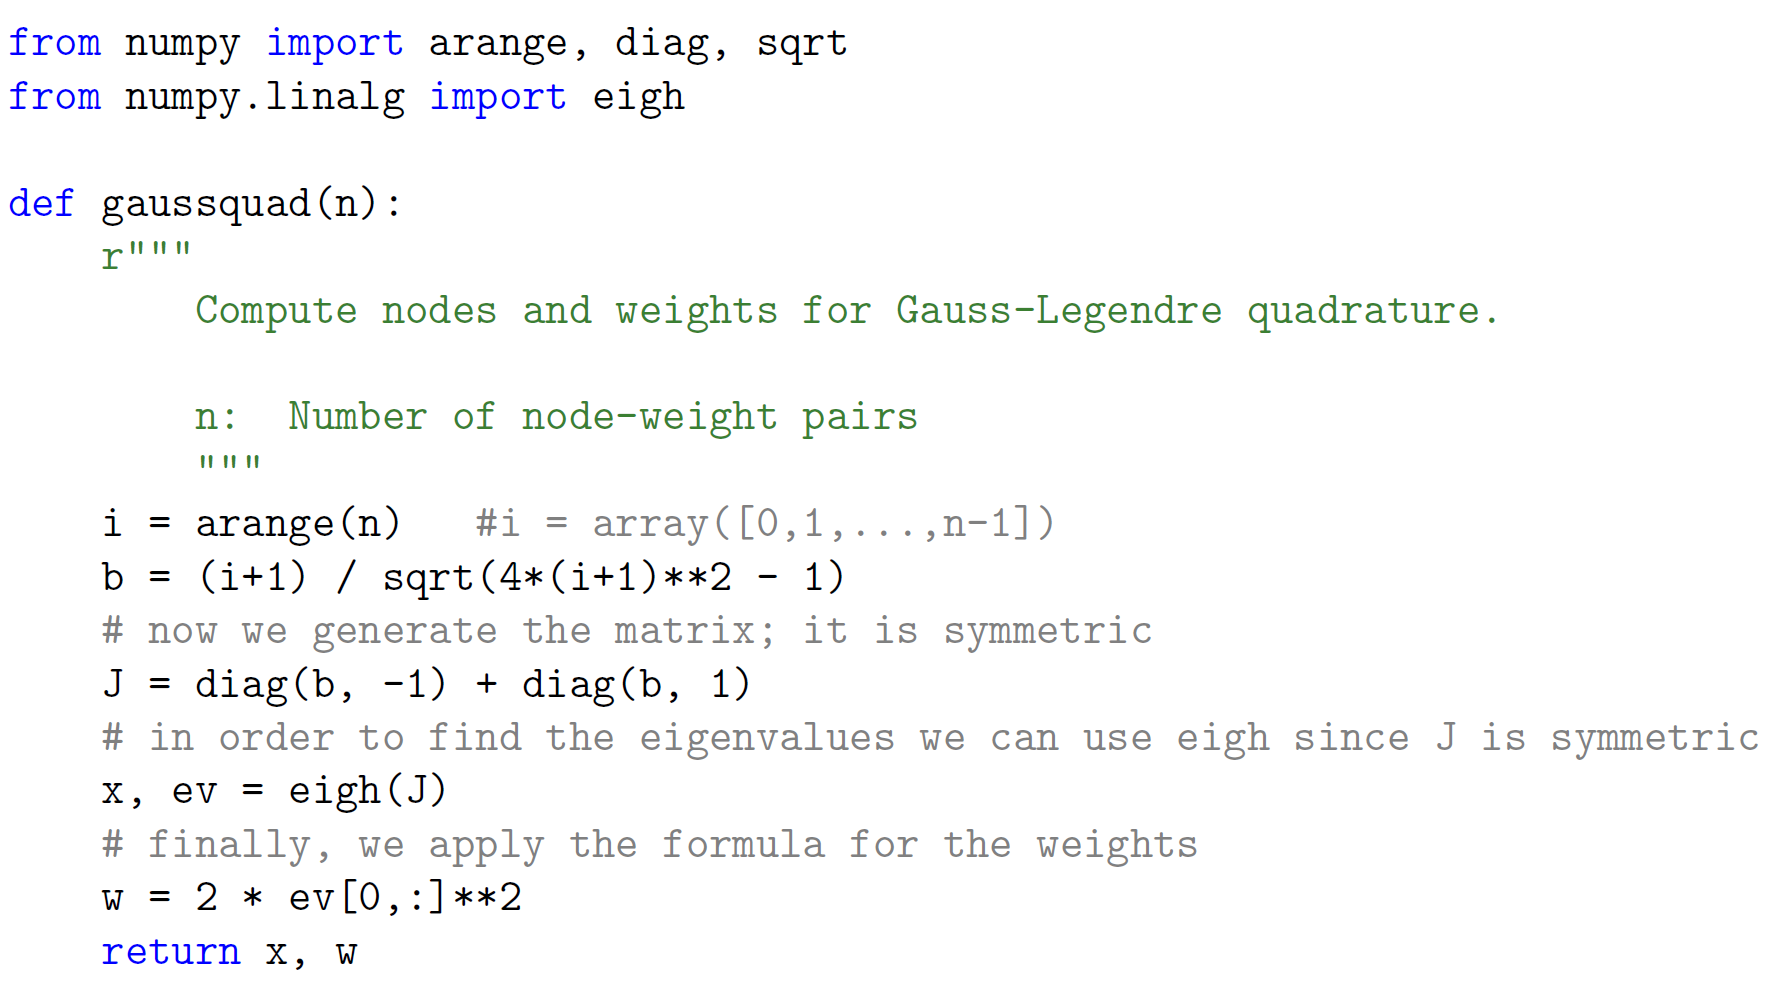
\includegraphics[width=0.3\textwidth]{Figures/Gauss_Legegendre.png}

        Skript Seite 16
    \end{center}    
}

\vspace{1\baselineskip}

\fat{Clenshaw-Curtis Formel} {

    Wir substituieren:
    \begin{align*}
        \int_{-1}^1 f(x) dx = \int_0^{\pi} f(\cos(\theta)) \sin(\theta) d \theta
        = \sum_{\text{k gerade}} \frac{2 a_k}{1-k^2}
    \end{align*}

    \begin{center}
        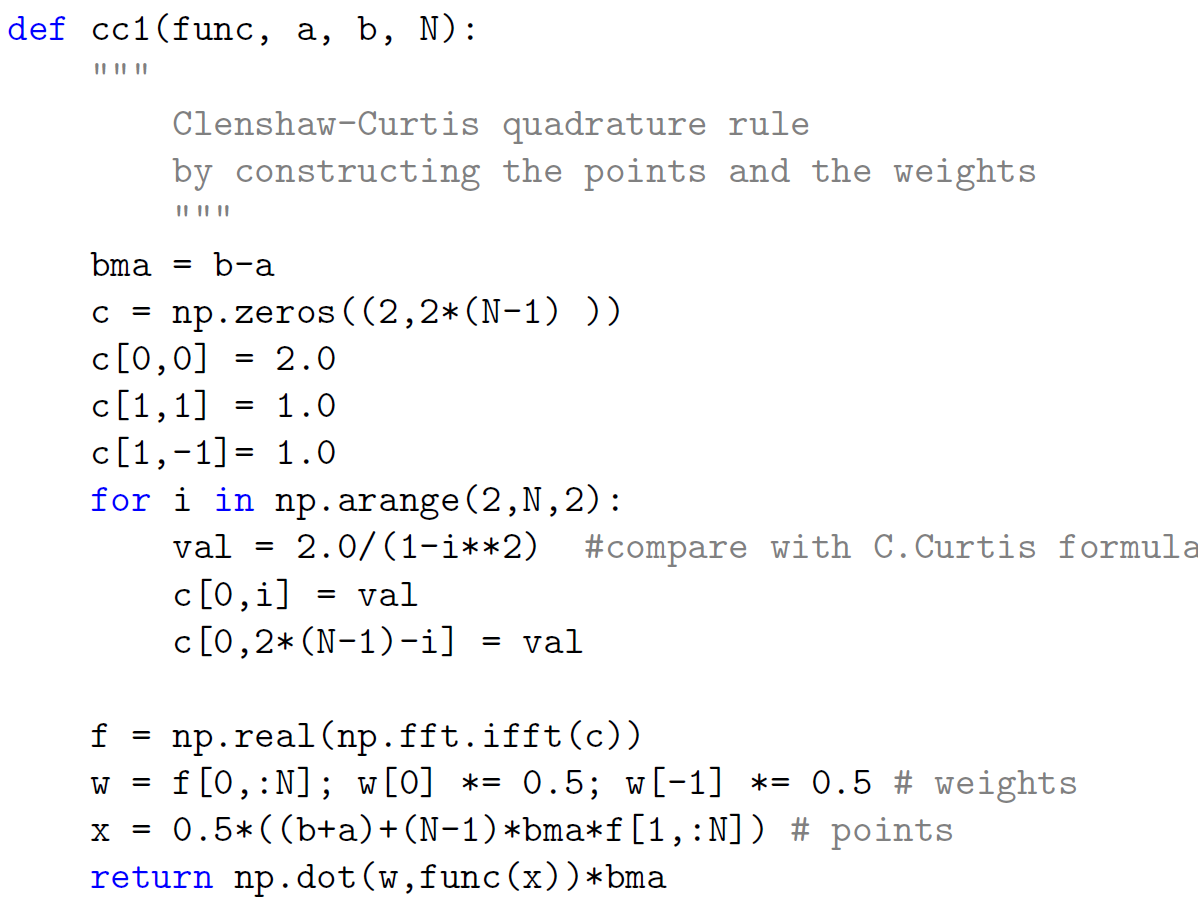
\includegraphics[width=0.4\textwidth]{Figures/cc1.png}

        Skript Seite 18
    \end{center}
    

    \begin{center}
        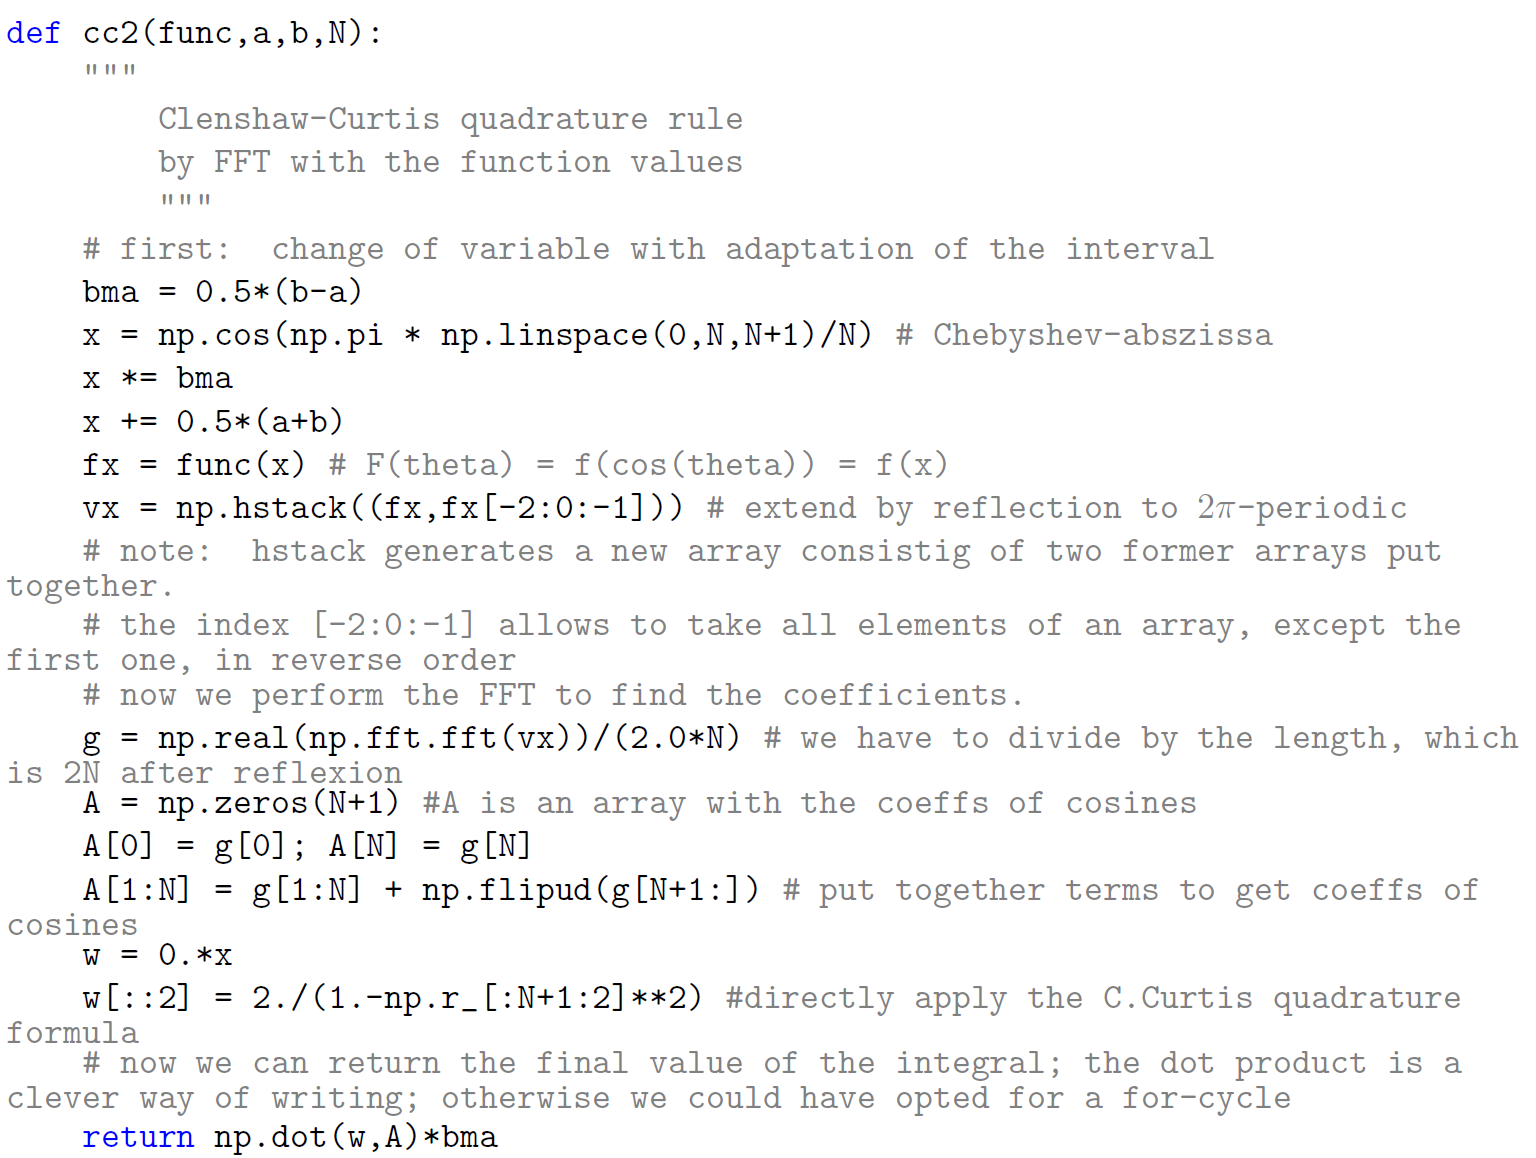
\includegraphics[width=0.5\textwidth]{Figures/cc2.png}

        Skript Seite 17
    \end{center}
}

\vspace{1\baselineskip}

\fat{Adaptive Quadratur}

    \begin{center}
        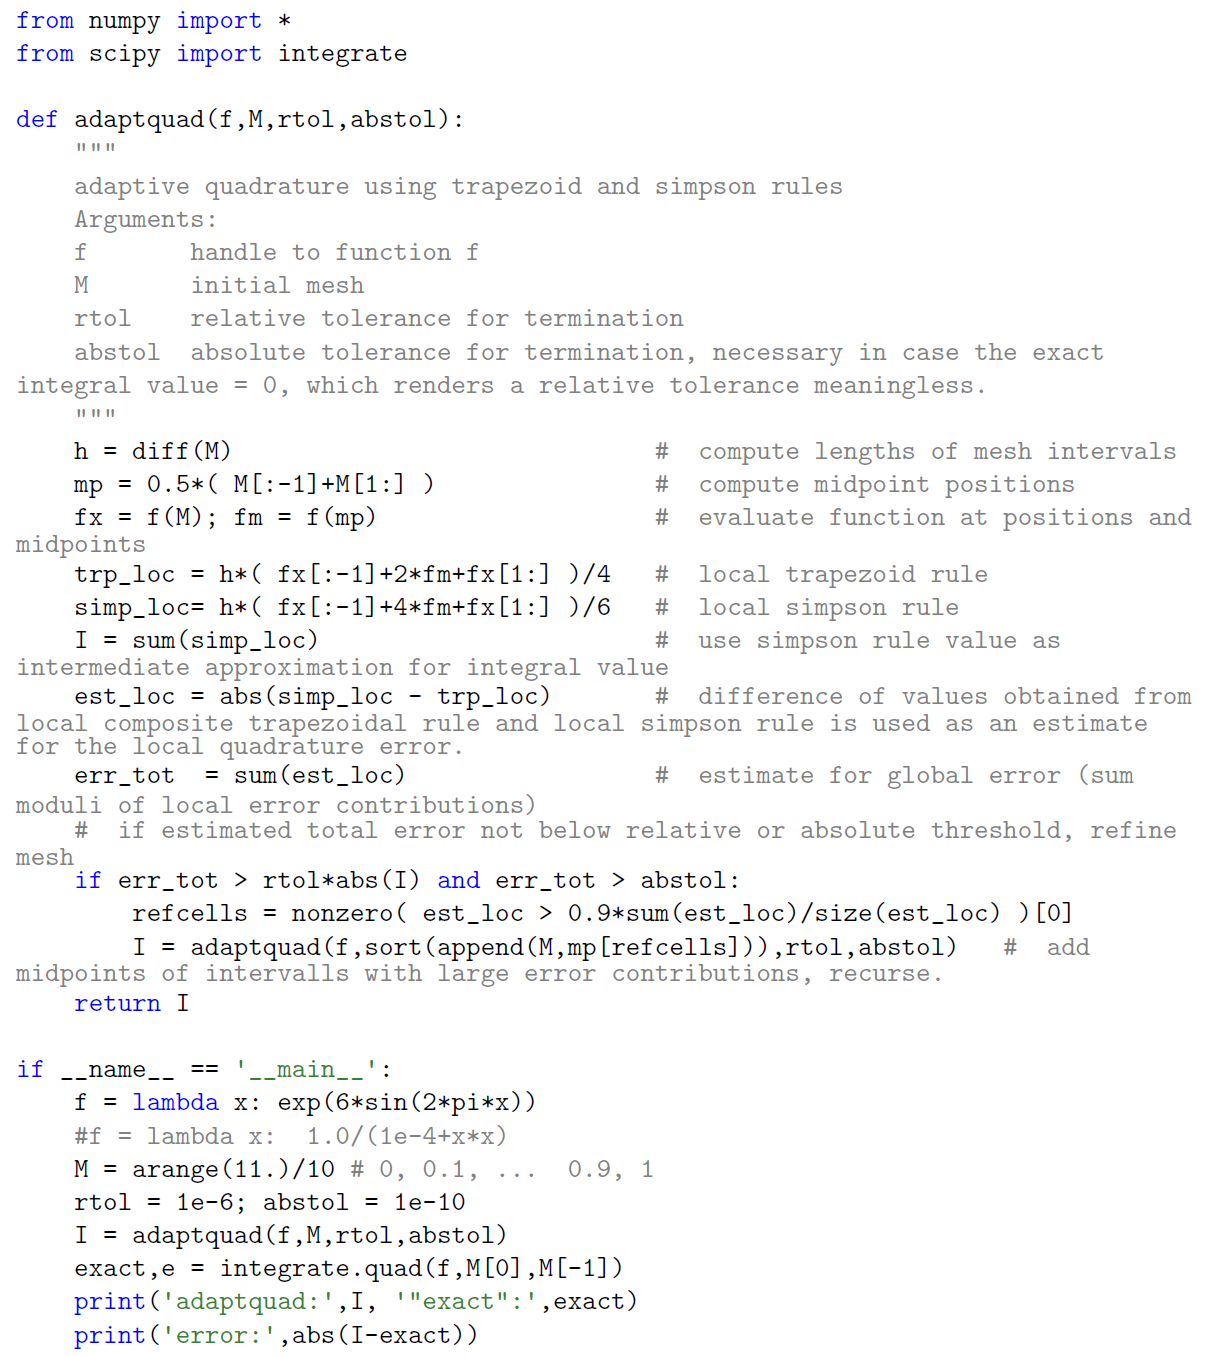
\includegraphics[width=0.4\textwidth]{Figures/AdaptQuad.png}

        Skript Seite 22
    \end{center}


\vspace{1\baselineskip}

\fat{Mehrdimensionale Integration} {

    Mit Satz von Fubini: eins nach dem anderen integrieren:
    \begin{align*}
        \int_{a_1}^{b_1} \dots \int_{a_d}^{b_d} f(x_1,\dots,x_d) dx_1 \dots dx_d
        \\
        \approx \sum_{i_1 = 0}^{n_1} \dots \sum_{i_d = 1}^{n_d} w_{i_1}^1 \dots w_{i_d}^{n_d} f(c_{i_1}^1 , \dots , c_{i_d}^d)
    \end{align*}
}

\vspace{1\baselineskip}

\fat{Python Code}:
\begin{itemize}
    \item Eindimensionale Integration: scipy.integrate.quad(f,a,b)[0]
    \item Mehrdimensionale Integration: 
    
            scipy.integrate.nquad(f,array([[a1,b1],\dots,[ad,bd]]))[0]
\end{itemize}

\vspace{1\baselineskip}

\fat{Drei Term Rekursion der Legendre Polynome}:
\begin{align*}
    P_{k+1} (x) = \klammer{x- \frac{\scalprod{x \cdot P_k}{P_k}}{\scalprod{P_k}{P_k}}} \cdot P_{k} (x)
        -  \klammer{\frac{\scalprod{P_k}{P_k}}{\scalprod{P_{k-1}}{P_{k-1}}}} P_{k-1} (x)
\end{align*}
Mit $P_0 (x) =1$ und $P_{-1} (x) = 0$
 
\vspace{1\baselineskip}

\Definition{

    Wir definieren die \fat{Lagrange-Polynome} für die Stützstellen $x_1,\dots,x_n$
    als
    \begin{align*}
        l_i (x) = \prod_{\stackrel{j=0}{i \neq j}} \frac{x-x_j}{x_i - x_j}
    \end{align*}
    Für diese gelten:
    \begin{enumerate}
        \item $l_i (x_j) = \delta_{ij}$
        \item $\grad \  l_i = n$
        \item $\sum_{i=0}^{n} l_i (x) = 1 \ \forall x \in \R$
        \item $\sum_{i=0}^{n} l_i^{(m)} (x) = 0$ für $m \geq 1$
        \item $l_1,\dots,l_n$ bilden eine Basis im Raum der Polynome von Grad $\leq n$.
    \end{enumerate}
}

\vspace{1\baselineskip}

\fat{Drei Term Rekursion der Lagrange Polynome}
\begin{align*}
    x P_{k-1} (x) = \frac{c_k}{a_k} P_{k-2} (x) - \frac{b_k}{a_k} P_{k-1} (x) + \frac{1}{a_k} P_{k} (x)
\end{align*}
Dies können wir in Matrixform bringen:
\begin{align*}
    A = \begin{pmatrix}
        - \frac{b_1}{a_1} & \frac{1}{a_1} & & & 0 \\
        \frac{c_2}{a_2} & - \frac{b_2}{a_2} & \frac{1}{a_2} & & \\
        & \ddots & \ddots & \ddots & \\
        & & \frac{c_{n-1}}{a_{n-1}} & \frac{b_{n-1}}{a_{n-1}} & \frac{1}{a_{n-1}} \\
        0 & & & \frac{c_n}{a_n} & \frac{b_n}{a_n}
    \end{pmatrix}
\end{align*}
Dies ist die gleiche Matrix wie bei der Gauss-Legendre Quadratur.
Sei $P_A$ das charakteristische Polynom von $A$. Dann sind die NST von $P_A$ die
Knotenpunkte der Gauss-Quadraturformel und die zu den jeweiligen Knotenpunkten
gehörigen Gewichte sind definiert als:
\begin{align*}
    w_j = \frac{1}{\Norm{v_j}}
\end{align*}
mit $v_j$ dem Eigenvektor zum Eigenwert $c_j$. Da diese aber nicht eindeutig sind,
muss normiert werden. Wir finden mit folgendem Verfahren die richtigen Eigenvektoren:
\begin{enumerate}
    \item Schreibe $u_j = c \cdot v_j = c \cdot [P_0 (t_j) , \dots , P_{n-1} (t_j)]^T$ für
            alle Eigenvektoren.
    \item Es muss gelten: $1=\scalprod{P_0}{P_0} = \int_{-1}^1 P_0 (t_1) P_0 (t_1) dx \
            \Longrightarrow P_0 (t_1) = \frac{1}{\sqrt{2}}$
    \item Wir betrachten den ersten Eintrag vom Eigenvektor: $(v_j)_1 = c \cdot P_0 (t_1) =
            c \cdot \frac{1}{\sqrt{2}} \ \Longrightarrow c = \sqrt{2} (v_j)_1$
    \item Man normiere alle Eigenvektoren: $v_j = \frac{1}{c} u_j = \frac{1}{\sqrt{2} (v_j)_1}
            v_j$
    \item Zum Schluss: $w_j = \frac{2 (v_j)_1^2}{\Norm{v_j}^2}$
\end{enumerate}

